

\part{Main Presentation}
	%****************************************************************************
	% Title Stuff
	%****************************************************************************
	%\frame{\titlepage}
	\begin{frame}
		\titlepage
	\end{frame}

	%****************************************************************************
	% Begin actual document content here
	%****************************************************************************

	\section{Quicksorts}
		\begin{frame}
			\frametitle{Introduction}
			\begin{itemize}
				\item<+-> $O(n \log(n))$ Average Case Run Time
				\item<+-> In place algorithm
				\item<+-> Picking Pivots
				\item<+-> Partitioning Data
				\item<+-> Recurse to a smaller sub-array
				\item<+-> Use Insertion Sort for a small sub-array
			\end{itemize}
			\note{
				Data is partitioned By Comparing and Swapping elements
			}
		\end{frame}	

		\subsection{Classic Quicksort}
			\begin{frame}
				\frametitle{Classic Quicksort}
				\begin{itemize}
					\item<+-> $2.13n \log n - 2.57n + O(\log(n))$ Comparisons
					\item<+-> $0.33n \log n - 0.58n + O(\log(n))$ Swaps
					\item<+-> One Pivot
					\begin{itemize}
						\item<+-> First Element
						\item<+-> Last Element
						\item<+-> Median of Three
					\end{itemize}
					\item<+-> Simple Partitioning
					\item<+-> Two Recursive Calls
				\end{itemize}
			\phantom{ }\cite{Wild:2012:ACA:2404160.2404231}
			\end{frame}
		
		\subsection{Dual Pivot Quicksort}
			\begin{frame}
				\frametitle{Dual Pivot Quicksort}
				\begin{itemize}
					\item<+-> $2n \log n - 1.51n + O(\log(n))$ Comparisons
					\item<+-> $0.8n \log n -0.3n + O(\log(n))$ Swaps
					\item<+-> Two Pivots
					\begin{itemize}
						\item<+-> First and Last Element
						\item<+-> Middle 2 of 5 elements (Evenly Spaced Out)
					\end{itemize}
					\item<+-> Partitions Smalls then Bigs (Middle is automatic)
					\item<+-> Three Recursive Calls
				\end{itemize}
				\phantom{ }\cite{Aumuller:2013:OPD:2525857.2525862}
				\note{
					Tertile Elements = Middle 2 of 5 elements (Evenly Spaced Out)
				}
			\end{frame}

		\subsection{Yaroslavskiy's Quicksort}
			\begin{frame}
				\frametitle{Yaroslavskiy's Dual Pivot Quicksort}
				\begin{itemize}
					\item<+-> $1.9n \log n - 2.46n + O(\log(n)$ Comparisons
					\item<+-> $0.6n \log n + 0.08n + O(\log(n))$ Swaps
					\item<+-> Two Pivots
					\begin{itemize}
						\item<+-> Middle 2 of 5 elements (Evenly Spaced Out)
						\item<+-> Uses 5-element sorting network
					\end{itemize}
					\item<+-> Simple Simultaneous Partition algorithm
					\item<+-> Two Recursive Calls 
				\end{itemize}
				\phantom{ }\cite{Wild:2012:ACA:2404160.2404231}
			\end{frame}
		
		\subsection{Three Pivot Quicksort}
			\begin{frame}
				\frametitle{Kushagra-Ortiz-Qiao-Munro Tri-Pivot Quicksort}
				\begin{itemize}
					\item<+-> $1.846n \log n + O(n)$ Comparisons
					\item<+-> $0.615n \log n + O(n)$ Swaps
					\item<+-> Three Pivots
					\begin{itemize}
						\item<+-> Middle 3 of 7 elements (Evenly Spaced Out)
					\end{itemize}
					\item<+-> Simultaneous Partition algorithm
					\item<+-> Four Recursive Calls 
				\end{itemize}
				\phantom{ }\cite{kushagra2013multi}
				\note{
					This algorithm had incomplete pseudo-code.
					Only the partition algorithm was specified.
				}
			\end{frame}
		
		\subsection{M-Pivot Quicksort}
			\begin{frame}
				\frametitle{M-Pivot Quicksort}
				\begin{itemize}
					\item<+-> $O(n \log n)$ Comparisons
					\item<+-> $O(n \log n)$ Swaps
					\item<+-> $M$ Pivots
					\begin{itemize}
						\item<+-> Sort $2M$ elements
					\end{itemize}
					\item<+-> Partition each segment on at a time 
					\item<+-> $M+1$ Recursive Calls
				\end{itemize}
				\phantom{ }\cite{kushagra2013multi}
			\end{frame}
		
			\begin{frame}
				\frametitle{Example M-Pivot Selection and Partitioning}
				\begin{center}   
					\includegraphics<1>[width=70mm]{MPivotSelectCanadates.png}
					\label{fig:MPivotSelectCanadates}
				\end{center}

				\begin{center}   
					\includegraphics<2>[width=72mm]{MPivotSelection.png}
					\label{fig:MPivotSelection}
				\end{center}

				\begin{center}   
					\includegraphics<3>[width=72mm]{MPivotPartiton.png}
					\label{fig:MPivotPartiton}
				\end{center}
				\phantom{ }\cite{kushagra2013multi}
			\end{frame}

			\begin{frame}
				\begin{itemize}
					\frametitle{Heap Optimized M-Pivot Quicksort}
					\item<+-> Enforce the Heap Property to the array before any computation
					\begin{itemize}
						\item<+-> Adds only $O(n)$ run time at each call
						\item<+-> Improves the sort to optimize pivot selection
					\end{itemize}
				\end{itemize}
				\phantom{ }\cite{kushagra2013multi}
			\end{frame}

			\begin{frame}
				\frametitle{Example M-Pivot Heap Optimized Pivot Selection}
				\begin{center}   
					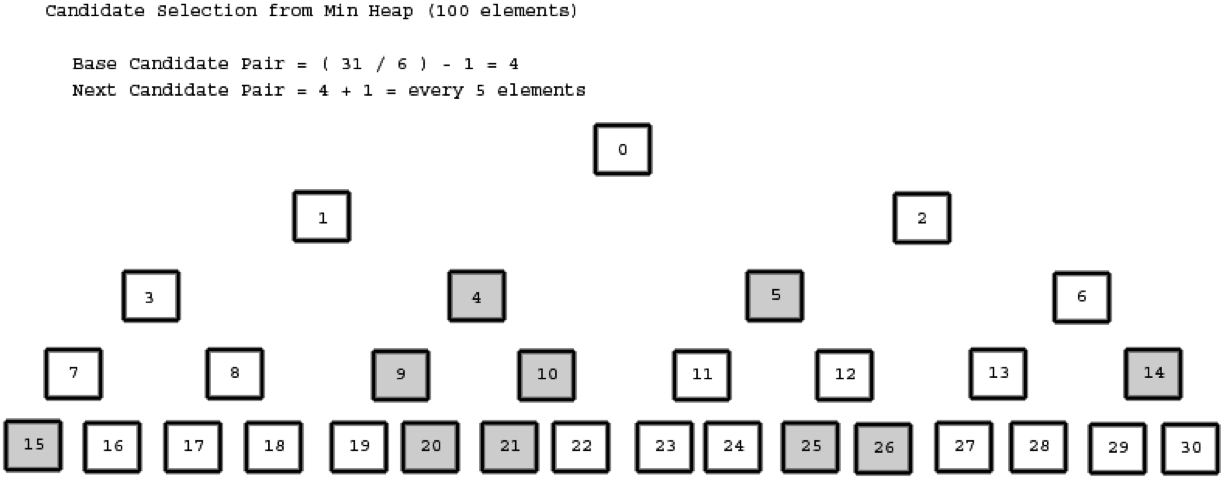
\includegraphics[width=100mm]{MPivotHeap.png}
					\label{fig:MPivotSelectCanadates}
				\end{center}
				\phantom{ }\cite{kushagra2013multi}
			\end{frame}

		\subsection{Summary}
			\begin{frame}
				\frametitle{Theoretical Average Case Run Time}
				\only<1>{
					\begin{center}
						\begin{tabular}{|r|l|}
							\hline
							Sort Method        &   Comparisons                          \\ \hline \hline
							Classic            &   $2n \log n - 1.51n  + O(\log(n))$   \\ \hline%\cite{Wild:2012:ACA:2404160.2404231}     \\ \hline
							Dual Pivot         &   $2.13n \log n - 2.57n + O(\log(n))$ \\ \hline%\cite{Wild:2012:ACA:2404160.2404231}     \\ \hline
							Optimal Dual Pivot &   $1.8n \log n + O(n)$               \\ \hline%\cite{Aumuller:2013:OPD:2525857.2525862} \\ \hline
							Three Pivot        &   $1.846n \log n + O(n)$             \\ \hline%\cite{kushagra2013multi}                 \\ \hline
							Yaroslavskiy       &   $1.9n \log n - 2.46n + O(\log(n)$  \\ \hline%\cite{Wild:2012:ACA:2404160.2404231}     \\ \hline
							M Pivot            &   $O(n \log n)$                        \\ 
							\hline
						\end{tabular}
					\end{center}
				}
				\only<2>{
					\begin{center}
						\begin{tabular}{|r|l|}
							\hline
							Sort Method         &     Swaps \\ \hline \hline
							Classic             &  $0.33n \log n - 0.58n + O(\log(n))$\\ \hline%\cite{Wild:2012:ACA:2404160.2404231}    \\ \hline
							Dual Pivot          &  $0.8n \log n -0.3n + O(\log(n))$   \\ \hline%\cite{Wild:2012:ACA:2404160.2404231}    \\ \hline
							Optimal Dual Pivot  &  $0.33n \log n + O(n)$              \\ \hline%\cite{Aumuller:2013:OPD:2525857.2525862}\\ \hline
							Three Pivot         &  $0.615n \log n + O(n)$             \\ \hline%\cite{kushagra2013multi}                \\ \hline
							Yaroslavskiy        &  $0.6n \log n + 0.08n + O(\log(n))$  \\ \hline%\cite{Wild:2012:ACA:2404160.2404231}    \\ \hline
							M Pivot             &  $O(n \log n)$ \\ 
							\hline
						\end{tabular}
					\end{center}				
				}
				\phantom{ }\cite{Aumuller:2013:OPD:2525857.2525862}\\
				\phantom{ }\cite{Wild:2012:ACA:2404160.2404231}\\
				\phantom{ }\cite{kushagra2013multi}
				\note{
					These are average case run times.
					The M-Pivot quicksort is not studied very well.
					As you see, people study each quicksort with a fixed number of pivots.
				}
			\end{frame}


	\section{Legend}
		\begin{frame}
			\frametitle{Legend}
			\begin{center}   
				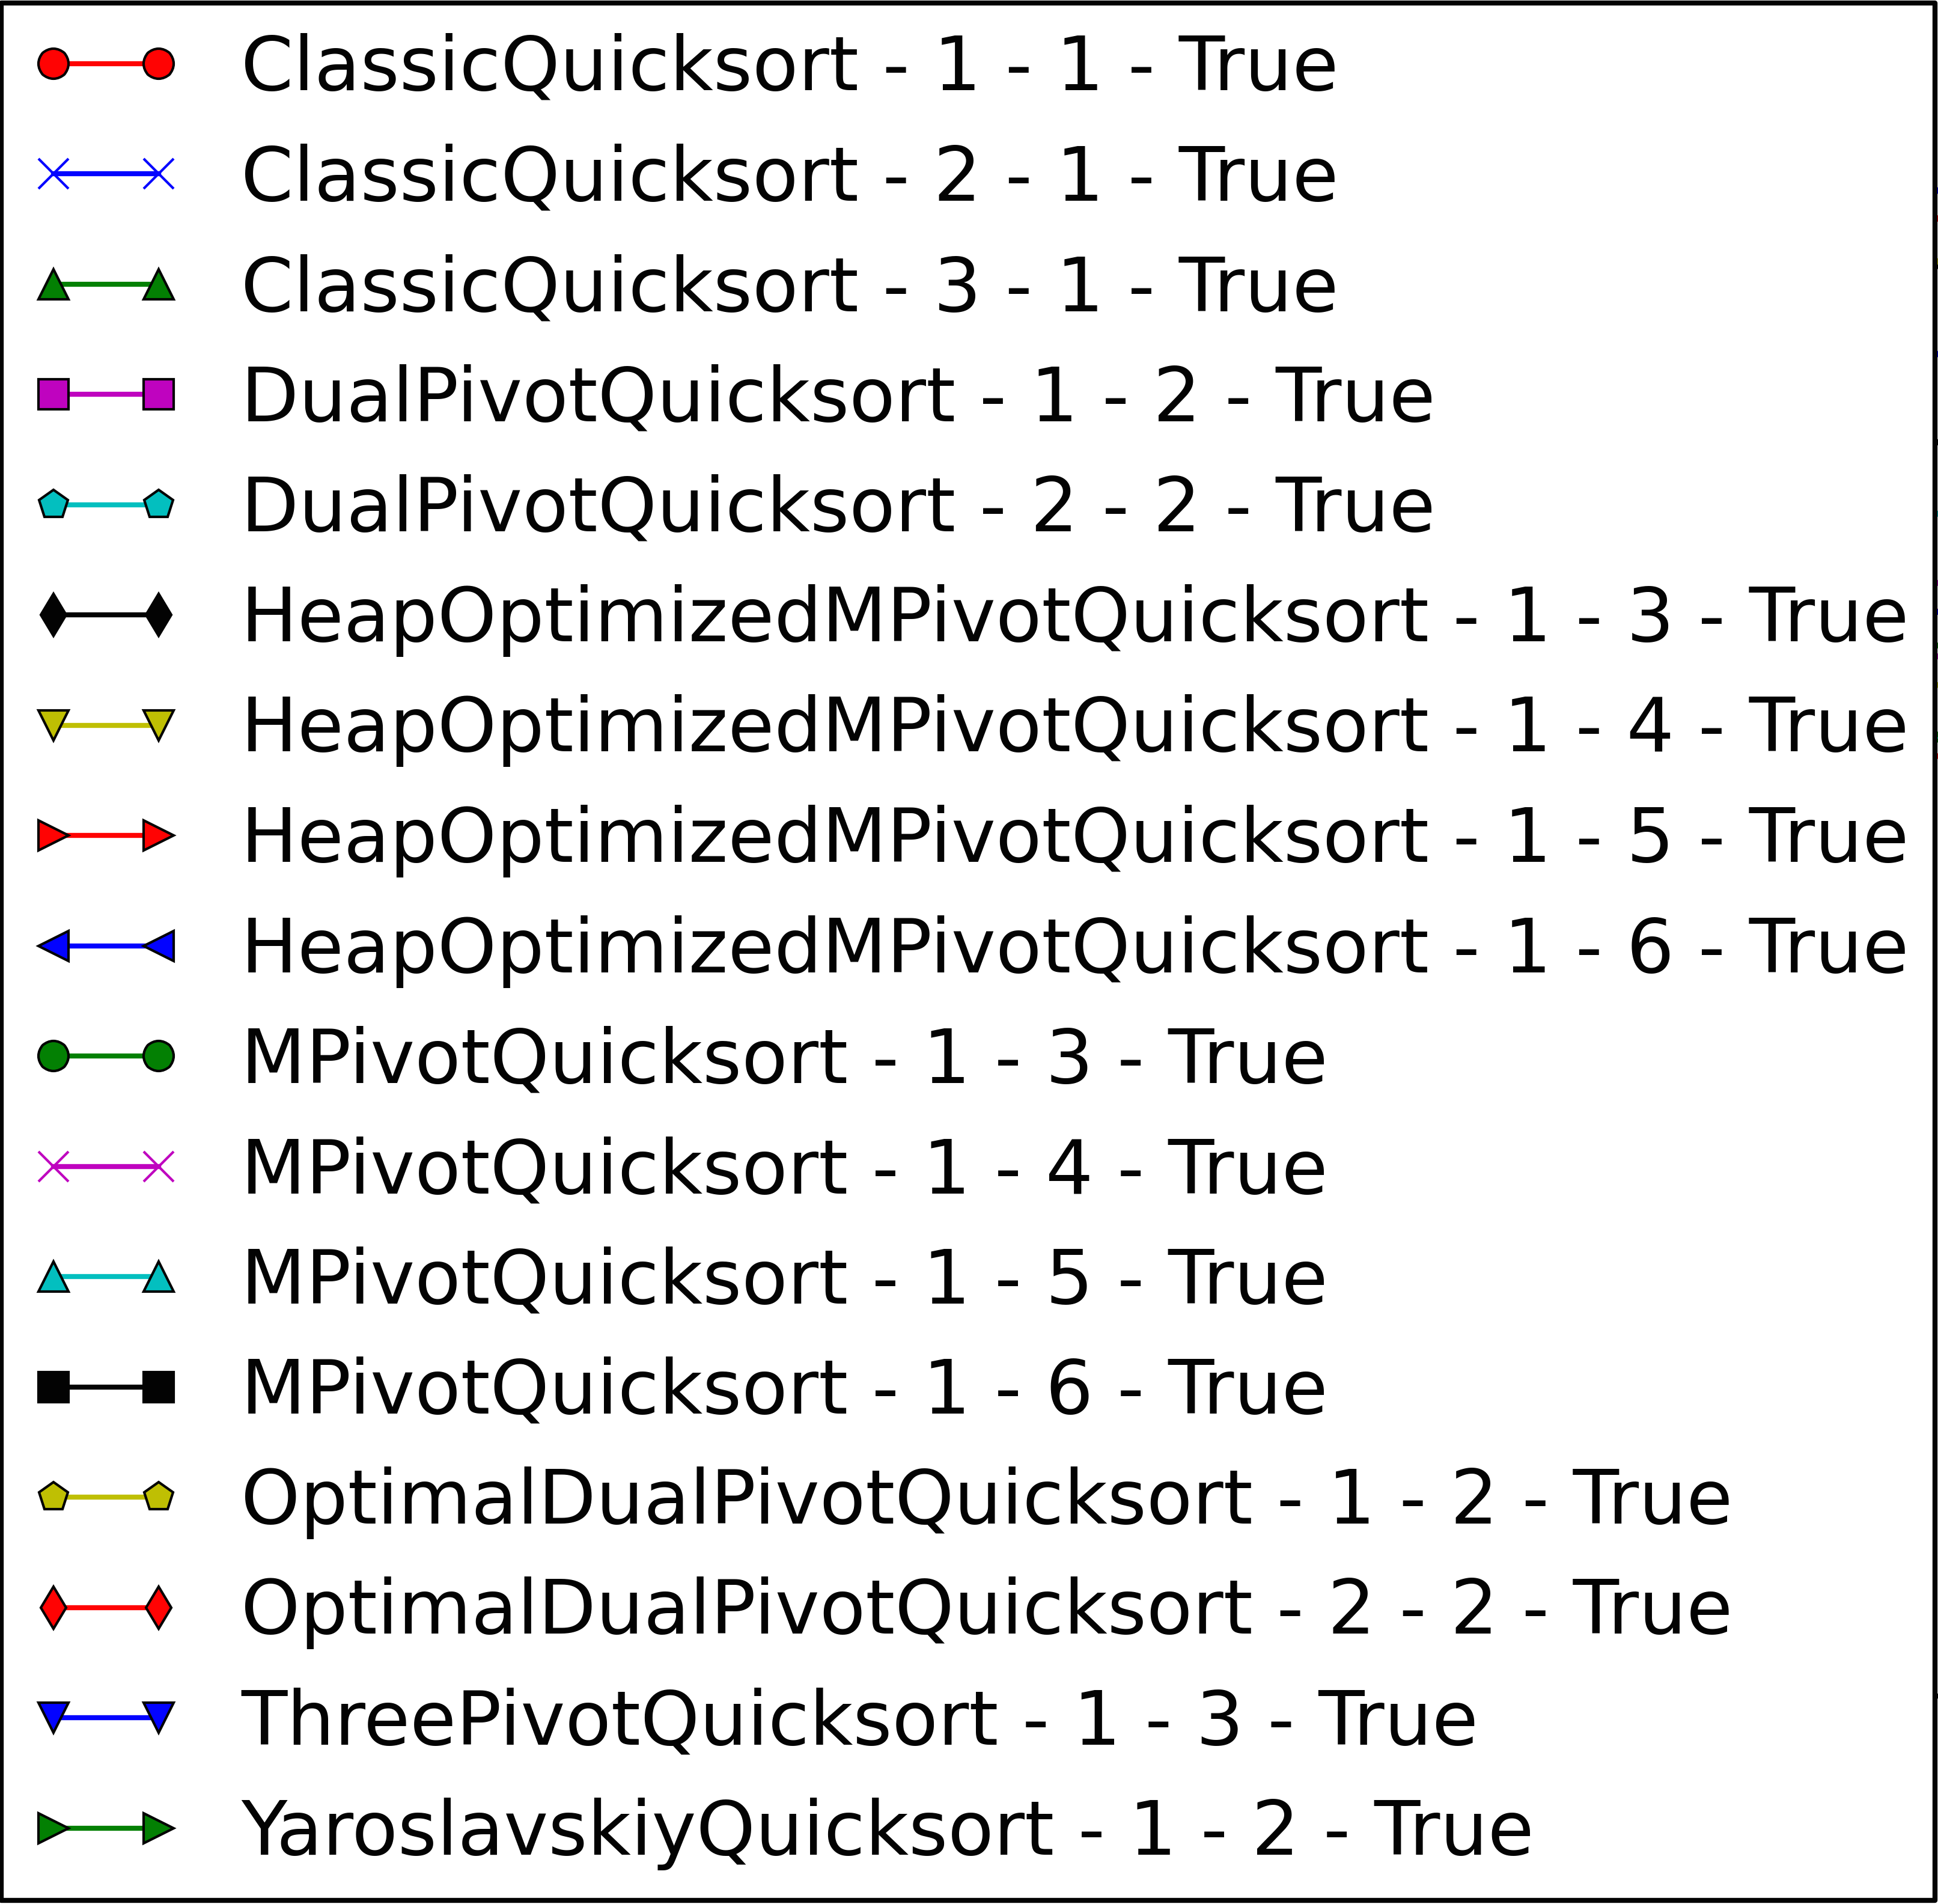
\includegraphics[width=72mm]{PlotLegend.png}
				\label{fig:PlotLegend}
			\end{center}
		\end{frame}

	\section{Results}
		\subsection{Mass Comparison}
			\begin{frame}
				\frametitle{Mass Comparison Small Scale}
				\begin{center}   
					\includegraphics<1>[width=75mm]{AllthePlotsSmallScale_comp.png}
				\end{center}
				
				\begin{center}   
					\includegraphics<2>[width=75mm]{AllthePlotsSmallScale_swap.png}
				\end{center}
			\end{frame}

			\begin{frame}
				\frametitle{Mass Comparison Large Scale}

				\begin{center}   
					\includegraphics<1>[width=75mm]{AllthePlotsLargeScale_comp.png}
				\end{center}
				
				\begin{center}   
					\includegraphics<2>[width=75mm]{AllthePlotsLargeScale_swap.png}
				\end{center}

			\end{frame}

			\begin{frame}
				\frametitle{Mass Comparison Semi Log x}

				\begin{center}   
					\includegraphics<1>[width=75mm]{SemilogxAllPlotsLargeScale_comp.png}
				\end{center}
				
				\begin{center}   
					\includegraphics<2>[width=75mm]{SemilogxAllPlotsLargeScale_swap.png}
				\end{center}

			\end{frame}


		\subsection{One Pivot}
			\begin{frame}
				\frametitle{One Pivot Comparison Small Scale}

				\begin{center}   
					\includegraphics<1>[width=75mm]{OnePivotsSmallScale_comp.png}
				\end{center}
				
				\begin{center}   
					\includegraphics<2>[width=75mm]{OnePivotsSmallScale_swap.png}
				\end{center}
			\end{frame}

			\begin{frame}
				\frametitle{One Pivot Comparison Large Scale}

				\begin{center}   
					\includegraphics<1>[width=75mm]{OnePivotsLargeScale_comp.png}
				\end{center}
				
				\begin{center}   
					\includegraphics<2>[width=75mm]{OnePivotsLargeScale_swap.png}
				\end{center}

			\end{frame}


		\subsection{Two Pivots}
			\begin{frame}
				\frametitle{Two Pivot Comparison Small Scale}

				\begin{center}   
					\includegraphics<1>[width=75mm]{TwoPivotsSmallScale_comp.png}
				\end{center}
				
				\begin{center}   
					\includegraphics<2>[width=75mm]{TwoPivotsSmallScale_swap.png}
				\end{center}

			\end{frame}

			\begin{frame}
				\frametitle{Two Pivot Comparison Large Scale}

				\begin{center}   
					\includegraphics<1>[width=75mm]{TwoPivotsLargeScale_comp.png}
				\end{center}
				
				\begin{center}   
					\includegraphics<2>[width=75mm]{TwoPivotsLargeScale_swap.png}
				\end{center}
			\end{frame}

		\subsection{Three Pivots}
			\begin{frame}
				\frametitle{Three Pivot Comparison Small Scale}
				\begin{center}   
					\includegraphics<1>[width=75mm]{ThreePivotsSmallScale_comp.png}
				\end{center}
				
				\begin{center}   
					\includegraphics<2>[width=75mm]{ThreePivotsSmallScale_swap.png}
				\end{center}
			\end{frame}

			\begin{frame}
				\frametitle{Three Pivot Comparison Large Scale}
				\begin{center}   
					\includegraphics<1>[width=75mm]{ThreePivotsLargeScale_comp.png}
				\end{center}
				
				\begin{center}   
					\includegraphics<2>[width=75mm]{ThreePivotsLargeScale_swap.png}	
				\end{center}
			\end{frame}
			
		\subsection{M Pivots}
			\begin{frame}
				\frametitle{M Pivot Comparison Small Scale}
				\begin{center}   
					\includegraphics<1>[width=75mm]{M-PivotQuicksortsSmallScale_comp.png}
				\end{center}
				
				\begin{center}   
					\includegraphics<2>[width=75mm]{M-PivotQuicksortsSmallScale_swap.png}
				\end{center}
			\end{frame}

			\begin{frame}
				\frametitle{M Pivot Comparison Large Scale}
				\begin{center}   
					\includegraphics<1>[width=75mm]{M-PivotQuicksortsLargeScale_comp.png}
				\end{center}
				
				\begin{center}   
					\includegraphics<2>[width=75mm]{M-PivotQuicksortsLargeScale_swap.png}
				\end{center}
			\end{frame}

	\section{The End}

	%****************************************************************************
	% Reference frames/slides
	%****************************************************************************
	\begin{frame}[allowframebreaks]
		\frametitle{References}    
		\bibliographystyle{plainnat}
		\bibliography{../References/refer}
	\end{frame}

	\begin{frame}
		\begin{center}
			\Huge Questions?
		\end{center}
	\end{frame}

\part{Answers}
	\begin{frame}
		% Empty Frame
		\note{
			Will add slides to answer potential questions
		}
	\end{frame}


%****************************************************************************
% End of the contents of the document
% Items related to end of document
%****************************************************************************